\documentclass{protokol}
\leftheader{Měření absorbce světla}
\centerheader{Praktikum III}
\rightheader{Tomáš Derner}

\begin{document}

  \section*{Úkol}

    \begin{enumerate}
      \item Ověřte platnost Beerova zákona pro různé tloušťky přiloženého pevného materiálu.
      \item Změřte absorpční spektrum přiložených vzorků skleněných filtrů. Diskutujte procento maximální propustnosti a spektrální šířku propouštěné oblasti.
      \item Spočtěte odrazivost $R$ povrchů skleněných ploch s indexem lomu $ n = \num{1.516}$, $\num{1.6}$ a $\num{1.78}$ a srovnejte s odrazivostí vzorků z úkolu 1.
      \item Proveďte odhad chyby transmitance a určete chybu nepřímého měření absorpčního koeficientu.
    \end{enumerate}

  \section*{Teorie}

    Absorpci světla homogenní látkou popisuje Lambertův-Beerův zákon
    \begin{equation} \label{eq:theta_i}
      \theta_i = 10^{\kappa l},
    \end{equation}
    kde $l$ je tloušťka vrstvy látky, $\kappa$ je absorpční koeficient a $\theta_i$ je vnitřní transmitance, tedy poměr světelného toku látkou prošlého vůči toku na látku dopadajícímu, pakliže neuvažujeme ztráty toku odrazem.

    Odraz však může mít na množství prošlého toku poměrně značný vliv, proto zavádíme transmitanci
    \begin{equation} \label{eq:theta}
      \theta \approx (1 - R)^2 \theta_i,
    \end{equation}
    kde $R$ je je odrazivost povrchu. Vztah platí při zanedbání mnohonásobných odrazů.

    Záporně vzatý dekadický logaritmus vnitřní transmitance nazýváme absorbancí 
    \begin{equation} \label{eq:A}
      A = - \log \theta_i = \kappa_l.
    \end{equation}

    Pro kolmý dopad světla na skleněnou desku plyne z Fresnelových vzorců výraz pro odrazivost 
    \begin{equation} \label{eq:R}
      R = \frac{(n-1)^2}{(n+1)^2},
    \end{equation}
    kde $n$ je index lomu skla.
  
  \newpage
  \section*{Výsledky}

    \subsection*{Úkol 1}

      Pomocí spektrometru \textbf{SPEKOL} byly změřeny relativní hodnoty světelných toků, které procházely skleněnými filtry. Vždy byl měřen tok určitým počtem čirých filtrů, kde se tok ztrácí jen odrazem, a shodným počtem zelených filtrů. Tento způsob měření umožnil eliminovat vliv odrazivosti na výsledný prošlý tok. Poměry těchto hodnot, tedy odpovídající vnitřní transmitance, jsou uvedeny v tabulce \ref{tab:u1}. Tyto hodnoty jsou pak proloženy exponenciálním fitem $\theta_i = Ae^{Bm}$ ($m$ je počet filtrů) a zobrazeny v grafech \ref{fig:u1_l450} až \ref{fig:u1_l600}. 

      \begin{table}[H]
        \centering
        \setlength{\tabcolsep}{10pt}
        \begin{tabular}[t]{
  lSSSSSSSSSSSSSSSSSSSSS
}\toprule
x [mm] & 1.3 & 1.2 & 1.2 & 1.3 & 1.2 & 1.2 & 1.2 & 1.3 & 1.2 & 1.2 & 1.3 & 1.2 & 1.2 & 1.3 & 1.2 & 1.2 & 1.2 & 1.3 & 1.2 & 1.2 & 1.3 \\\bottomrule
\end{tabular}
        \caption{Hodnoty vnitřních transmitancí pro různé vlnové délky světla}
        \label{tab:u1}
      \end{table}

      \begin{figure}[H]
        \centering
        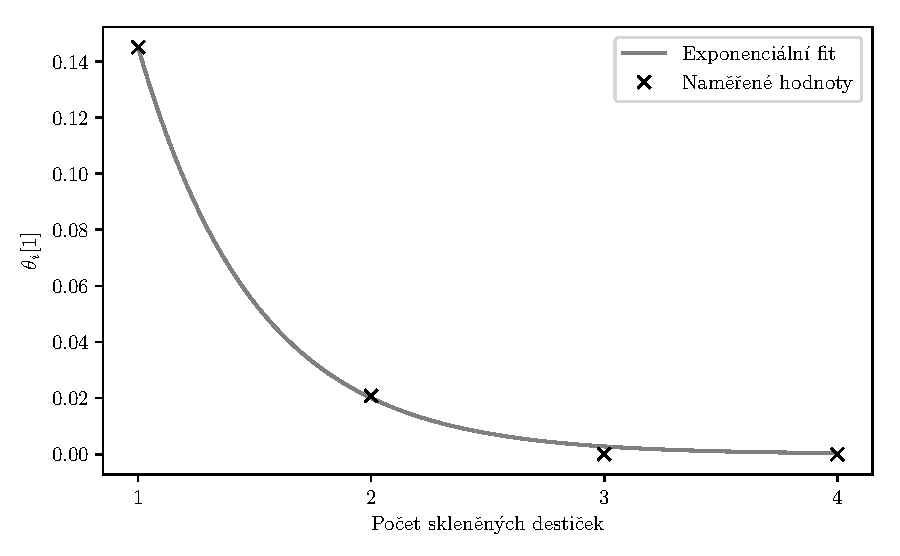
\includegraphics[]{u1_l450}
        \caption{Závislost vnitřní transmitance na počtu skleněných filtrů pro $\lambda = \SI{450}{nm}$}
        \label{fig:u1_l450}
      \end{figure}

      \begin{figure}[H]
        \centering
        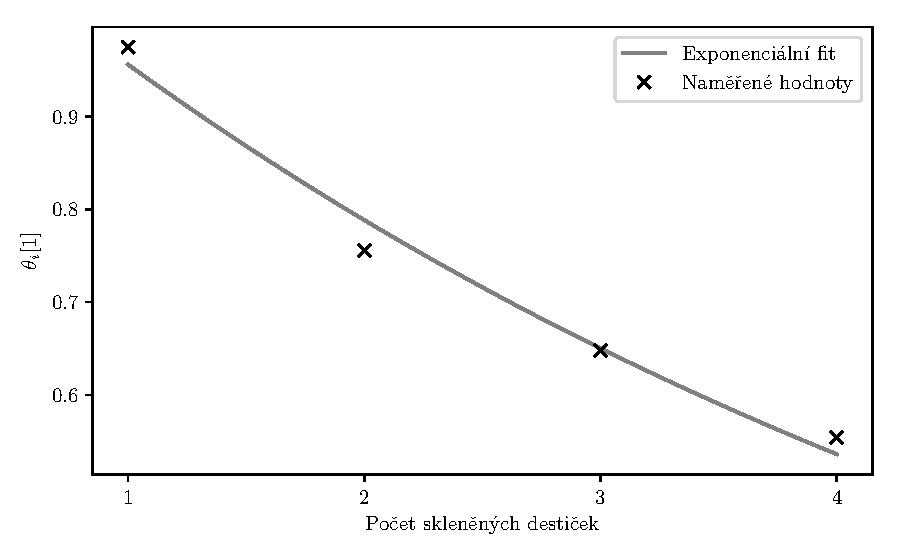
\includegraphics[]{u1_l520}
        \caption{Závislost vnitřní transmitance na počtu skleněných filtrů pro $\lambda = \SI{520}{nm}$}
        \label{fig:u1_l520}
      \end{figure}

      \begin{figure}[H]
        \centering
        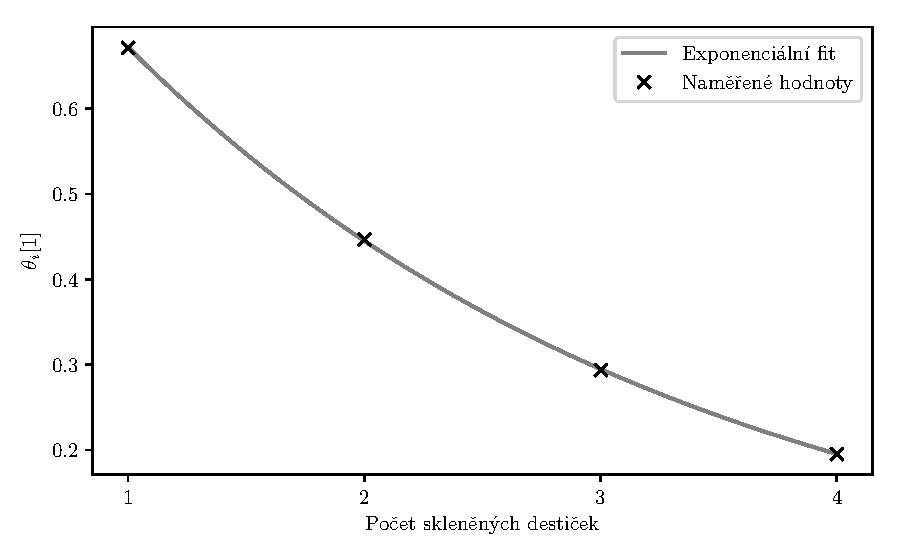
\includegraphics[]{u1_l600}
        \caption{Závislost vnitřní transmitance na počtu skleněných filtrů pro $\lambda = \SI{600}{nm}$}
        \label{fig:u1_l600}
      \end{figure}

      Koeficienty regresí jsou
      $$ A^{\SI{450}{nm}} = \num{1.05 \pm 0.11}, $$
      $$ B^{\SI{450}{nm}} = \num{-1.97 \pm 0.10}, $$
      $$ A^{\SI{520}{nm}} = \num{1.16 \pm 0.05}, $$
      $$ B^{\SI{520}{nm}} = \num{-0.19 \pm 0.02}, $$
      $$ A^{\SI{600}{nm}} = \num{1.015 \pm 0.003}, $$
      $$ B^{\SI{600}{nm}} = \num{-0.412 \pm 0.002}. $$

    \subsection*{Úkol 2}

      Vláknovým spektrometrem \textbf{Vernier} byla proměřena absorpční spektra různých skleněných filtrů jako závislost absorbance $A$ na vlnové délce $\lambda$, výsledek je zanesen v grafu \ref{fig:u2}.

      \begin{figure}[H]
        \centering
        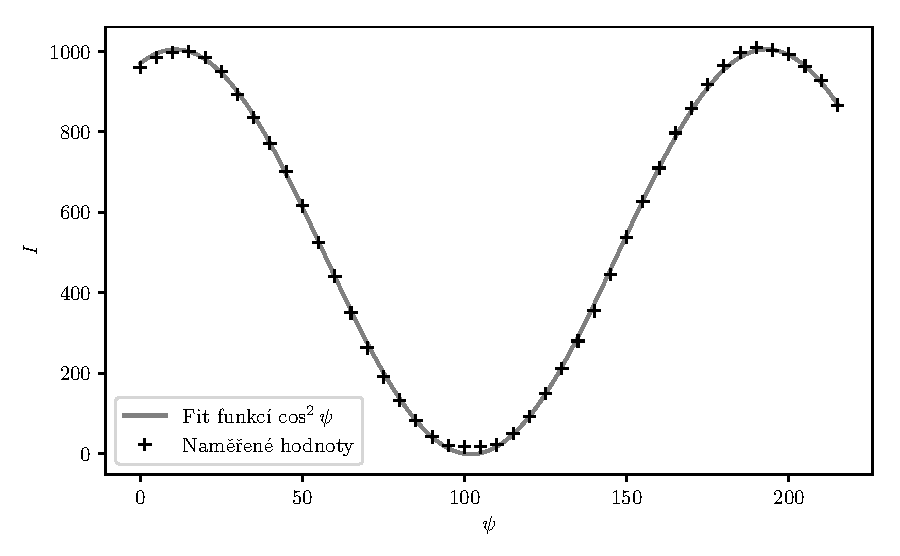
\includegraphics[]{u2}
        \caption{Absorpční spektra pro různé skleněné filtry}
        \label{fig:u2}
      \end{figure}

    \subsection*{Úkol 3}
      
      Pomocí vztahu \eqref{eq:R} spočteme odrazivost pro index lomu $n_1 = \num{1.516}$
      $$ R_1 = \num{0.0421}, $$
      pro $n_2 = \num{1.6}$
      $$ R_2 = \num{0.0533} $$
      a pro $n_3 = \num{1.78}$
      $$ R_3 = \num{0.0787}.$$

      Během řešení úkolu 1 byl měřen také prošlý světelný tok čirým skleněným filtrem vůči dopadajícímu, výsledné transmitance jsou uvedeny v tabulce \ref{tab:u3}.

      \begin{table}[H]
        \centering
        \setlength{\tabcolsep}{10pt}
        \begin{tabular}[t]{
  S[table-format=1.0]
  S[table-format=1.2]
  S[table-format=1.2]
  S[table-format=1.2]
}\toprule
{počet filtrů} & {$\theta^{\SI{450}{nm}}$}   & {$\theta^{\SI{520}{nm}}$}   & {$\theta^{\SI{600}{nm}}$}  \\\midrule
1              & 0.940                       & 0.980                       & 0.933                      \\
2              & 0.890                       & 0.920                       & 0.880                      \\
3              & 0.840                       & 0.880                       & 0.840                      \\
4              & 0.805                       & 0.830                       & 0.787                      \\\bottomrule
\end{tabular}

        \caption{Hodnoty transmitancí pro čiré filtry}
        \label{tab:u3}
      \end{table}

      Pomocí rovnice \eqref{eq:theta} spočteme odrazivosti 
      $$ R^{\SI{450}{nm}} = \num{0.0304 \pm 0.0003}, $$
      $$ R^{\SI{520}{nm}} = \num{0.0101 \pm 0.0001}, $$
      $$ R^{\SI{450}{nm}} = \num{0.0341 \pm 0.0003}. $$

  \section*{Diskuse}
    
    Z grafů \ref{fig:u1_l450} a \ref{fig:u1_l600} v úkolu 1 je zřejmě vidět exponenciální závislost transmitance na počtu filtrů, potažmo na tloušťce materiálu. Naměřené hodnoty v grafu \ref{fig:u1_l520} vykazují také zhruba exponenciální průběh, avšak exponenciální fit nesedí těmto hodnotám příliš dobře a má téměř lineární charakter, což bylo pravděpodobně způsobeno chybou při měření.

    Naměřené průběhy závislosti absorbance na vlnové délce odpovídají pro jednotlivé barvy filtrů intuici a ačkoli se v průběhu odpovídající zelenému filtru objevují jisté nefyzikální oscilace, nevyskytují se v měření žádné nespojitosti či poruchy. V tomto úkolu se do výsledků měření mohla drobně promítnout skutečnost, že otvor spektrometru pro vložení měřeného vzorku není dobře odstíněn od okolního světla.

    Měřená závislost transmitance na počtu čirých filtrů se zanedbatelnou vnitřní transmitancí ukazuje, že mezi jednotlivými skleněnými destičkami vznikaly drobné vzduchové mezery, na kterých se realizovaly další odrazy a tedy ztráty světelného toku. Proto byla pro výpočet odrazivosti použita vždy hodnota odpovídající jednomu sklíčku. Srovnáním hodnot odrazivosti získaných z měření transmitance a vypočtených ze zadaných indexů lomu vidíme, že použitým destičkám odpovídá nejlépe index lomu $n_1 = \num{1.516}$. Výrazná odchylka hodnot měření při použité vlnové délce $\SI{520}{nm}$ opět ukazuje na možnou hrubou chybu během tohoto měření.

  \section*{Závěr}

    Pomocí spektrometru \textbf{SPEKOL} byla ověřena platnost Lambertova-Beerova zákona.

    Spektrometrem \textbf{Vernier} byly měřeny absorpční spektra několika barevných filtrů.

    Srovnáním odrazivostí získaných z měření transmitance a vypočtených ze zadaných indexů lomu byla určena nejlepší shoda indexu lomu použitého skla s indexem lomu $n_1 = \num{1.516}$.

  \begin{thebibliography}{}

    \bibitem{mereni}
    Studijní text "Měření absorpce světla", dostupné z\\ \url{http://physics.mff.cuni.cz/vyuka/zfp/_media/zadani/texty/txt_317.pdf}, 21.\,3.\,2017
  
  \end{thebibliography}

\end{document}